\makeatletter\def\input@path{{minimus}{notebook-neon}}\makeatother

\documentclass{notebook-neon}

\usepackage{minimus-section}
\usepackage{minimus-text}
\usepackage{minimus-math}
\usepackage{minimus-float}
\usepackage{minimus-code}
\usepackage{minimus-colorbox}
\usepackage{minimus-tikz}
\usepackage{minimus-reference}
\usepackage{minimus-bibtex}

\graphicspath{{build}{image}}
\lstset{inputpath={code}}

\title{计算机体系结构}
\author{李宇轩}

\begin{document}

\maketitle

\frontmatter

\makesymb

\begin{center}
    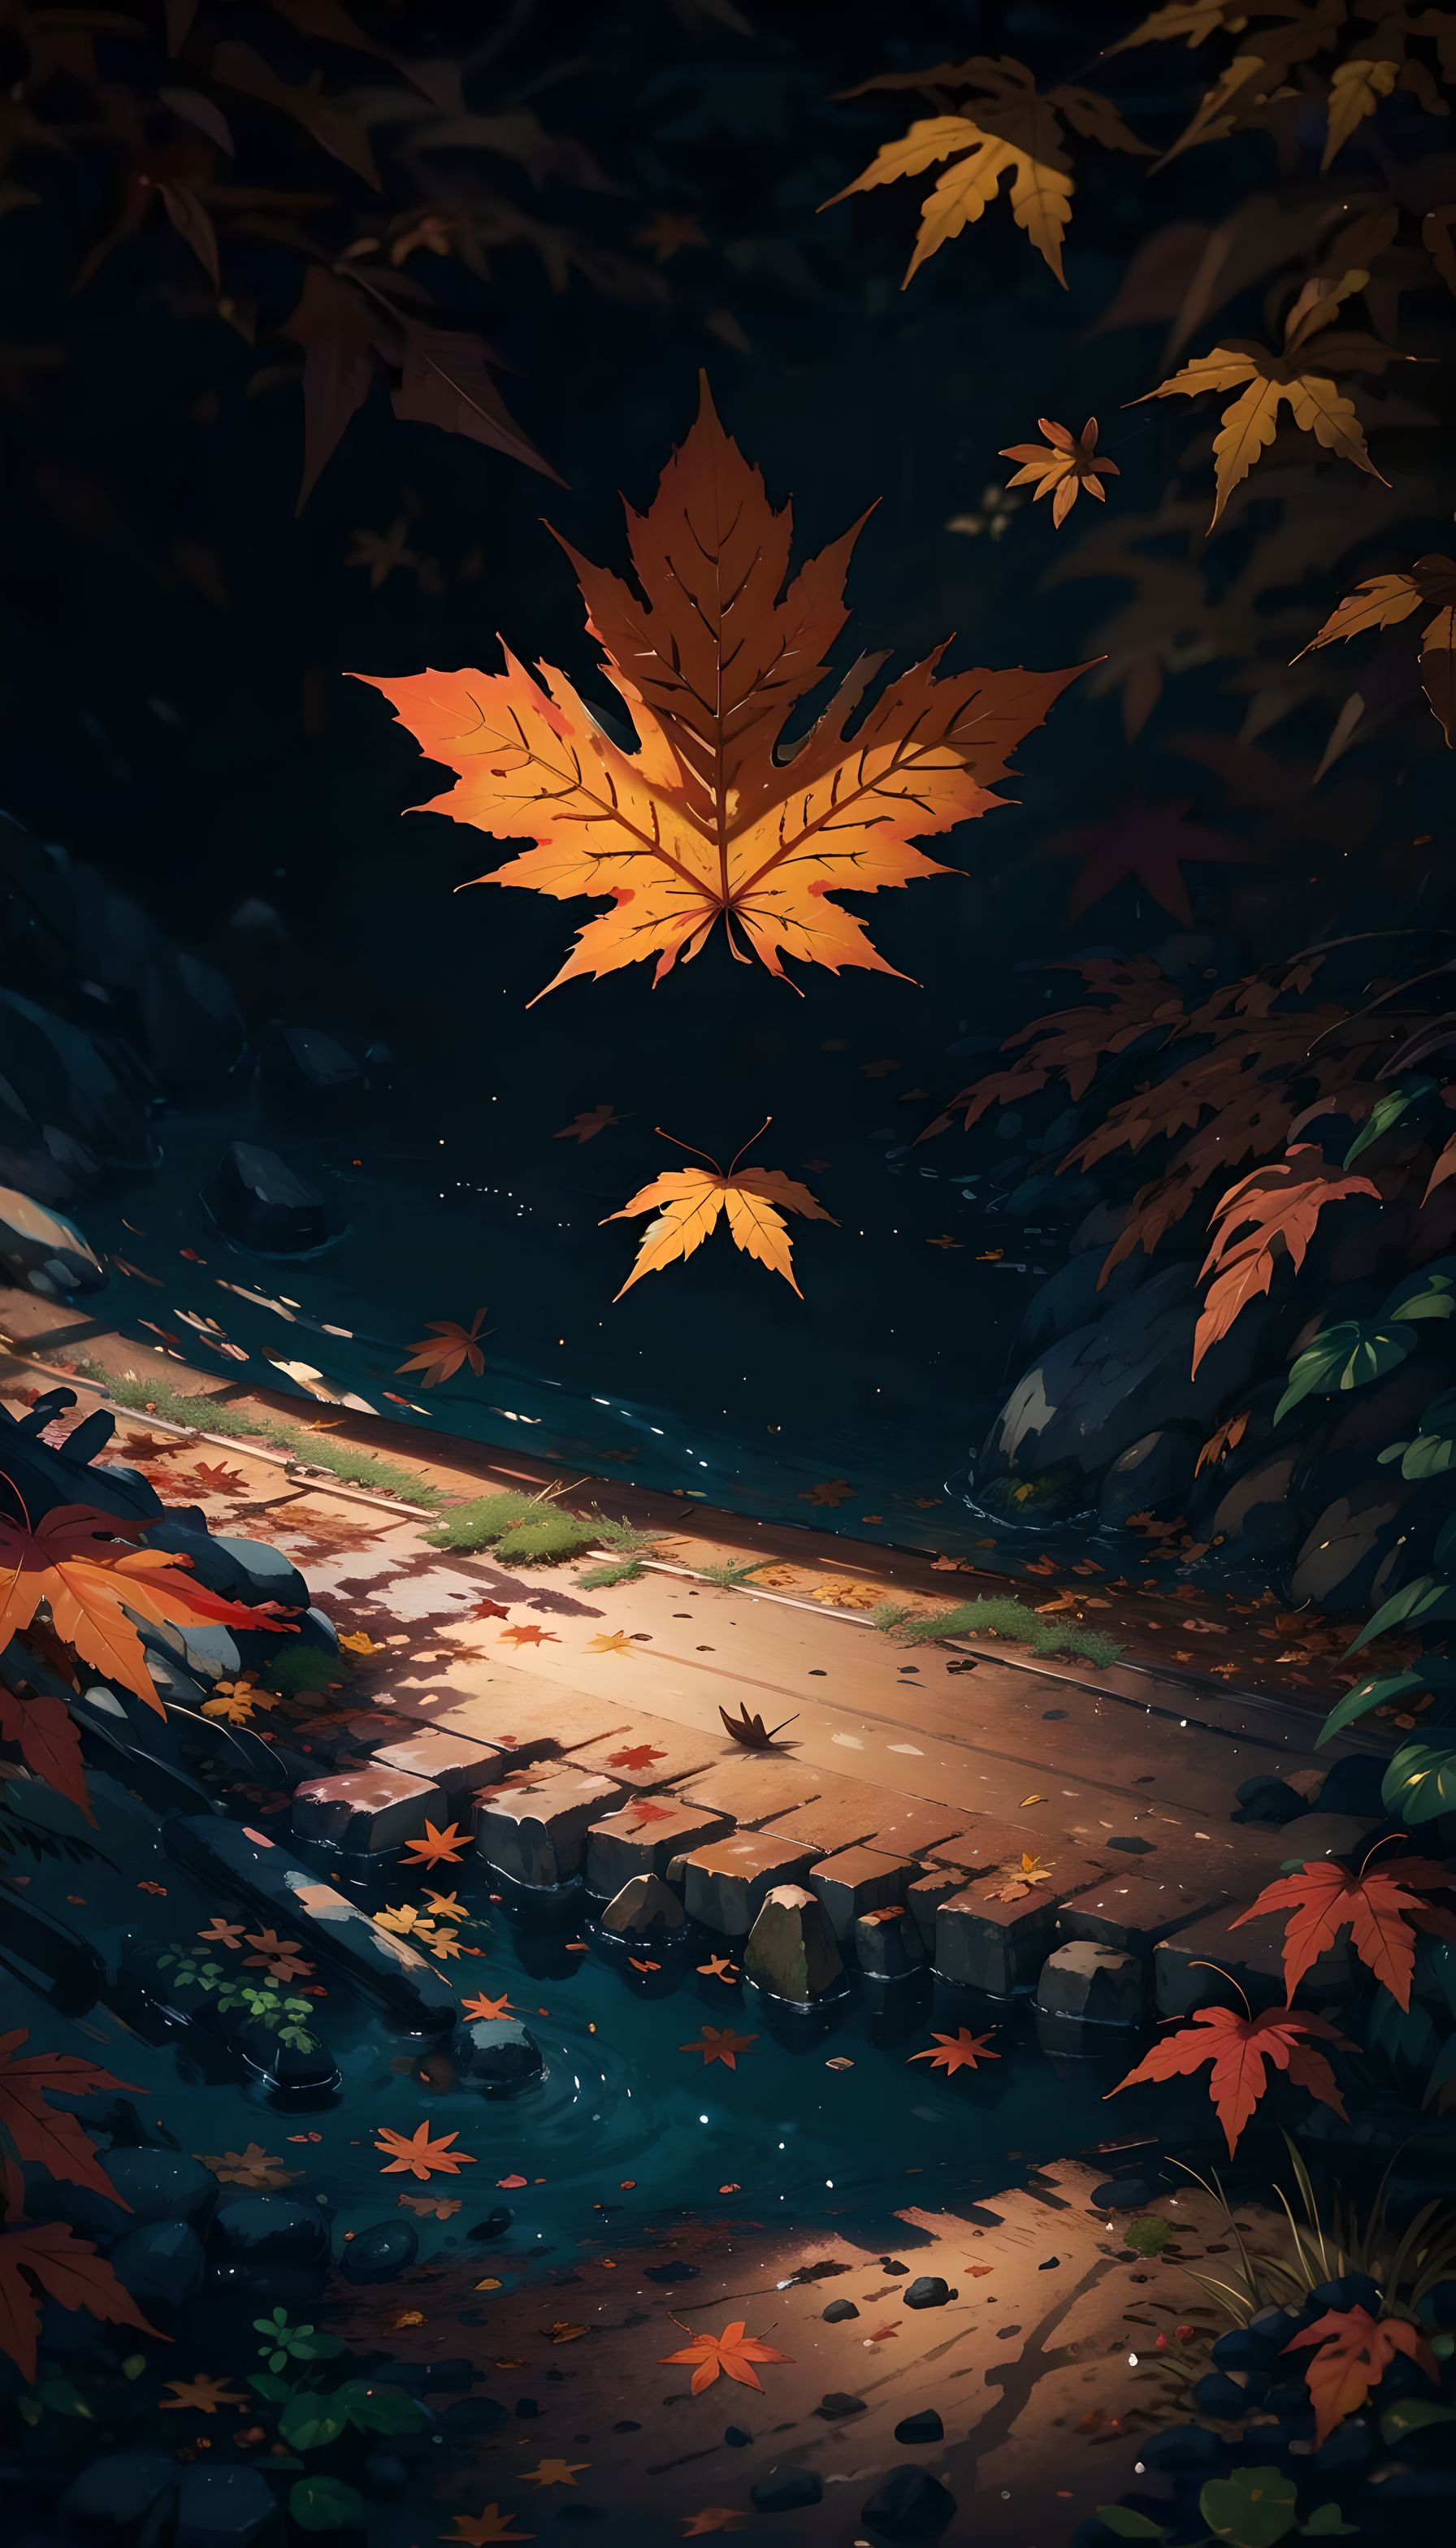
\includegraphics[width=13.5cm]{019.jpeg}
\end{center}

\clearpage

\tableofcontents
\listoffigures
\listoftables
\lstlistoflistings

\mainmatter

\nocite{*}

\chapter{RISC-V指令集架构}

在计算机体系结构中,我们会用术语架构(Architecture)和微架构(Microarchitecture)来指代“指令集架构”和“处理器架构”。指令集架构描述处理器要实现哪些指令,处理器架构描述处理器具体实现指令的硬件电路。现有的指令集包含x86、ARM、MIPS、RISC-V等,显然同一套指令集可以有多个不同的硬件实现,例如Intel和AMD都有x86指令集架构的处理器,它们可以运行相同的程序,但是具有不同的底层电路。本章和下一章将分别研究RISC-V指令集和处理器,不同于闭源的x86和ARM,RISC-V是一个迅速发展的新兴开源指令集。

在本章,我们将讨论汇编语言(Assembly Language)、机器语言(Machine Language)、编译器和汇编器的基本原理。我们知道,汇编语言是很接近硬件指令的语言,其语句几乎是和硬件指令一一对应的,这一部分我们主要会研究我们熟悉的高级语言的特性(运算、条件语句、循环语句、数组、函数)在汇编语言层面是怎么实现的,换言之,就是要研究处理器到底是怎么通过一条条简单的指令来实现这一切的。机器语言中指令都以二进制表示了,以供处理器运行。这一部分我们主要研究指令应当如何由二进制表示。最后,我们会讨论高级语言编写的代码是如何通过编译器和汇编器最终变成可执行程序,以及程序是以何种方式被处理器运行。

\section{汇编语言}

\subsection{汇编指令的基本概念}

在计算机中,最简单的操作就是加法运算,在\cref{code:高级语言中的加法}和\cref{code:汇编语言中的加法}中,分别展示了高级语言(C语言)和汇编语言中加法的写法。汇编语言中用\code{#}表示注释,而不是C语言的\code{//}或\code{/**/}。

\begin{Code}[高级语言中的加法]{c}
    \lstinputlisting{Chapter06A_01.cod.c}
\end{Code}

\begin{Code}[汇编语言中的加法]{riscv}
    \lstinputlisting{Chapter06A_02.cod.asm}
\end{Code}

而减法和加法是完全类似的,如\cref{code:高级语言中的减法}和\cref{code:汇编语言中的减法}所示。\goodbreak

\begin{Code}[高级语言中的减法]{c}
    \lstinputlisting{Chapter06A_03.cod.c}
\end{Code}

\begin{Code}[汇编语言中的减法]{riscv}
    \lstinputlisting{Chapter06A_04.cod.asm}
\end{Code}

汇编指令分为两部分,其中\code{add}和\code{sub}称为指令的助记符(Mnemonic),代表要执行什么操作,而\code{a,b,c}则称为指令的操作数(Operand),\code{a}是目标操作数,\code{b,c}是源操作数,指令会对源操作数进行计算并将结果写入目标操作数。当然,实际上这里直接写\code{a,b,c}是不符合汇编语法的,在汇编层面没有“变量”这样的东西。我们之后会具体介绍操作数可以是什么。

这里不管加法还是减法,对于操作数的格式都是相同的,这蕴含了下面的原则。
\begin{BoxDesignPrinciple}[规律性即简洁性]
    \centering
    Regularity supports simplicity.
\end{BoxDesignPrinciple}

而对于一些更复杂的计算,例如\cref{code:高级语言中的复杂计算}和\cref{code:汇编语言中的复杂计算}中,我们需要计算的是\code{a=b+c-d},汇编会将其变为两条指令,先计算\code{b+c}并将中间结果暂存在\code{t}中,再通过计算\code{t-d}即\code{b+c-d}得到\code{a} 。
\begin{Code}[高级语言中的复杂计算]{c}
    \lstinputlisting{Chapter06A_05.cod.c}
\end{Code}

\begin{Code}[汇编语言中的复杂计算]{riscv}
    \lstinputlisting{Chapter06A_06.cod.asm}
\end{Code}

这里用多条汇编指令实现复杂操作的思想蕴含了RISC-V的另一条设计原则。
\begin{BoxDesignPrinciple}[令通常情形更快]
    \centering
    Make the common case fast.
\end{BoxDesignPrinciple}

实际上,是否为这样的复合任务设置专门的指令,区分了两类不同的指令集
\begin{itemize}
    \item 复杂指令集(CISC, Complex Instruction Set Computer)
    \item 简单指令集(RISC, Reduced Instruction Set Computer)
\end{itemize}
x86是一个典型的复杂指令集,有一个典型的例子是,x86中会为“字符串拷贝”设置一个专门的指令,这在简单指令集中可能需要上百条指令才能完成,然而,这样的复杂指令带来的硬件开销会降低简单指令的执行速度,违背“令通常情形更快”的设计原则。RISC-V则是一个简单指令集。简单指令集通过控制指令数量,使硬件复杂度和所需的指令编码长度最小化。

\subsection{算数指令}

指令的操作数在实践中会有两种情形:寄存器、立即数。
\begin{itemize}
    \item 寄存器:代表变量
    \item 立即数:代表常量
\end{itemize}

首先来解释寄存器,我们或许会认为通过一条\code{add a,b,c}的指令可以从内存中读取\code{b,c}相加并写入\code{a}处。然而事实是,指令无法直接访问内存!这是因为内存的读写速度远远慢于处理器执行指令的速度。在处理器内部,有一个称为寄存器堆(Register Set)的结构,对于RISC-V处理器,寄存器堆由32个寄存器构成,这些寄存器读写都非常快,可以被指令直接访问。

这里我们看到,容量越小的存储单元往往意味着比较快的读写速度。
\begin{BoxDesignPrinciple}[越小越快]
    \centering
    Smaller is faster.
\end{BoxDesignPrinciple}
\cref{fig:RISC-V寄存器堆结构}展示了RISC-V寄存器堆的结构,其包含的32个寄存器可以依次用\code{x0,x1,...,x31}来表示。然而,这32个寄存器并非完全相同可以自由使用的,而是被分配了特定的功能
\begin{itemize}
    \item 1个零寄存器(Zero Register):\code{zero}
    \item 1个返回地址寄存器(Return Address Register):\code{ra}
    \item 1个栈指针寄存器(Stack Pointer Register):\code{sp}
    \item 1个全局指针寄存器(Global Pointer Register):\code{gp}
    \item 1个线程指针寄存器(Thread Register):\code{tp}
    \item 6个临时寄存器(Temporary Register):\code{t0,t1,t2,t3,t4,t5}
    \item 8个参数寄存器(Argument Register):\code{a0,a1,a2,a3,a4,a5,a6,a7}
    \item 12个保存寄存器(Saved Register):\code{s0,s1,s2,s3,s4,s5,s6,s7,s8,s9,s10,s11}
    \item \code{s0} 亦可兼作帧指针寄存器(Frame Pointer Register),可用\code{fp}表示。
    \item \code{a0,a1} 亦可兼作返回值寄存器(Return Values Register)。
\end{itemize}

在汇编语言中,我们更常用的是上面由功能命名的寄存器名称,而不是\code{x0,x1,...,x31}。

这些不同寄存器的具体作用和差异我们会在后文逐渐揭示。眼下,我们可以当成一般变量使用的是保存寄存器\code{s0,s1,...,s11}和临时寄存器\code{t0,t1,...,t5},另外,零寄存器\code{zero}也很有用,它被硬连线为$0$值,这意味着\code{zero}可以作为常数$0$被读取且对\code{zero}的写入无效。

\begin{Figure}[RISC-V寄存器堆结构]
    \includegraphics[scale=0.8]{Chapter06A_01.fig.pdf}
\end{Figure}

在\cref{code:RISC-V的寄存器加法指令}和\cref{code:RISC-V的寄存器减法指令}中,展示了加法指令和减法指令\code{add,sub}的操作,两者分别将\code{s1,s2}寄存器(假设寄存器\code{s1,s2}中已存有恰当的值)求和或求差,并将结果存入\code{s0}寄存器中。
\begin{Code}[RISC-V的寄存器加法指令]{riscv}
    \lstinputlisting{Chapter06A_07.cod.asm}
\end{Code}

\begin{Code}[RISC-V的寄存器减法指令]{riscv}
    \lstinputlisting{Chapter06A_08.cod.asm}
\end{Code}

在\cref{code:RISC-V的取负指令}中,展示了取负指令\code{neg}的操作,我们知道对一个数取负本质上等价于用零去减该数,即\code{neg s0,s1}等价于\code{sub s0 zero s1},因此硬件其实并没有必要实现取负指令的必要。

\begin{Code}[RISC-V的取负指令]{riscv}
    \lstinputlisting{Chapter06A_09.cod.asm}
\end{Code}

伪指令(Pseudoinstruction)是指具有类似指令的形式,但并不被处理器直接支持的语句。伪指令是为便利汇编语言编写而存在的,其往往是某一真正指令的特殊情况。伪指令会在汇编过程中按其定义转换为处理器支持的真正指令。\cref{code:RISC-V的取负指令}中的\code{neg}就是一条很典型的伪指令!

在C语言中,除了\code{a=b+c},我们还可能会使用\code{a=b+42}这样的语句。这里像\code{42}这样的数字并不需要被存储,而是在运算时立即被使用,这就是所谓的立即数(Immediate)。不过,虽然同样是加法,在汇编语言层面,寄存器加法\code{add}和立即数加法\code{addi}是两条不同的指令!在\cref{code:RISC-V的立即数加法指令}展示了立即数加法指令\code{addi}的使用,要注意的是,立即数必须放在后面的位置。另外在汇编代码中,立即数使用十六进制或十进制其实都是可以的(这里用了十六进制来表示)。
\begin{Code}[RISC-V的立即数加法指令]{riscv}
    \lstinputlisting{Chapter06A_10.cod.asm}
\end{Code}

立即数加法\code{addi}有很多作用,其中之一就是填充一个寄存器。不过应注意\code{addi}中的立即数只能是$12$位的,这是因为一条指令自身也只有$32$位,需要留一些空间给寄存器和指令编码。
\begin{Code}[RISC-V的立即数低位加载指令]{riscv}
    \lstinputlisting{Chapter06A_11.cod.asm}
\end{Code}

如何将完整的$32$位立即数加载到一个寄存器中呢?这需要组合使用立即数高位加载\code{lui}和立即数加法\code{addi},由\code{lui}指令加载高$20$位,由\code{addi}指令加载低$12$位,如\cref{code:RISC-V的立即数高位加载指令}所示。
\begin{Code}[RISC-V的立即数高位加载指令]{riscv}
    \lstinputlisting{Chapter06A_12.cod.asm}
\end{Code}

如何更优雅的实现这一点呢?伪指令\code{li}可以直接加载一个$32$位立即数至寄存器
\begin{itemize}
    \item 若\code{li}加载的立即数低于$12$位,则汇编为\code{addr}。
    \item 若\code{li}加载的立即数高于$12$位,则汇编为\code{lui}和\code{addr}的组合。
\end{itemize}

在\cref{code:RISC-V的立即数高位加载指令}中,展示了立即数加载伪指令\code{li}的使用,包含其两种可能的情况。
\begin{Code}[RISC-V的立即数加载指令]{riscv}
    \lstinputlisting{Chapter06A_13.cod.asm}
\end{Code}

立即数加法\code{addi}的第二个作用是通过对一个寄存器加\code{0}实现寄存器拷贝\code{mv}。
\begin{Code}[RISC-V的寄存器拷贝指令]{riscv}
    \lstinputlisting{Chapter06A_15.cod.asm}
\end{Code}

立即数加法\code{addi}的第三个作用是通过对\code{zero}加\code{0}实现空指令\code{nop}。空指令\code{nop}并不会有任何实际效果,如\cref{code:RISC-V的空指令}所示,但它会实实在在占有处理器的一个时钟周期,这在有些情况下是有用的,例如在C语言层面可以通过一定数量的\code{nop}实现\code{sleep()}这样的延时函数。
\begin{Code}[RISC-V的空指令]{riscv}
    \lstinputlisting{Chapter06A_14.cod.asm}
\end{Code}

\subsection{逻辑指令}

在\cref{code:RISC-V的逻辑指令}中展示了RISC-V的逻辑指令\code{and,or,xor}的用法,它们分别实现两个寄存器间的按位与、或、异或。类似于算数指令,这三者亦有对应的立即数版本\code{andi,ori,xori}。

我们可以从一个很有趣的角度考察这些逻辑运算。\cref{code:RISC-V的逻辑指令}中是对\code{s0,s1}进行逻辑运算并将结果保存在\code{s2}中。在这些逻辑运算中\code{s0,s1}是平等的,但不妨碍我们分别赋予它们一些不同的含义。若认为\code{s0}是\code{s1}的掩膜(mask),此时这三种逻辑运算可以理解为
\begin{itemize}
    \item 在\code{and}运算中,掩膜\code{s0}的效果是令\code{s1}中那些自身为\code{0}的位也被“清除”为\code{0}。
    \item 在\code{or }运算中,掩膜\code{s0}的效果是令\code{s1}中那些自身为\code{1}的位也被“赋值”为\code{1}。
    \item 在\code{xor}运算中,掩膜\code{s0}的效果是令\code{s1}中那些自身为\code{1}的位发生“翻转”。
\end{itemize}

我们或许注意到了一个问题,最基本的非运算\code{not}为什么还没有提及?实际上,这是因为非运算\code{not s2 s1}是\code{xori s2 s1 -1}对应的伪指令!结合上述对\code{xori}的直观理解很容易解释这点:依照补码规则,立即数\code{-1}意味着其每一位都是\code{1}。若将\code{-1}视为掩膜,它会令参与异或运算的另外一个数\code{s1}中每一位都发生翻转,显然,这就等价于对数\code{s1}进行非运算了。

\begin{Code}[RISC-V的逻辑指令]{riscv}
    \lstinputlisting{Chapter06A_16.cod.asm}
\end{Code}

目前,诸如\code{addi, xori}等的立即数运算指令中,立即数都被限制在$12$位以内。然而,立即数参与这些运算时,势必需要扩展到$32$位。一般的说,这类二进制数扩展有两种方式
\begin{itemize}
    \item 无符号扩展(Zero Extended),将高位用零填充。
    \item 有符号扩展(Sign Extended),将高位用原先的最高位填充。
\end{itemize}

立即数采用符号扩展,这也是为何前面$12$位下的\code{-1}扩展到$32$位时仍然是全\code{1}。

\subsection{移位指令}
在\cref{code:RISC-V的移位指令}中展示了RISC-V的移位指令\code{sll,srl,sra}以及\code{slii,srli,srai}的用法。
\begin{Code}[RISC-V的移位指令]{riscv}
    \lstinputlisting{Chapter06A_17.cod.asm}
\end{Code}

我们都知道,位移有“左移”和“右移”两种,但为何这里有三条位移指令?
\begin{itemize}
    \item \code{sll,slli}是逻辑左移,左移后低位的空位用\code{0}填充。
    \item \code{srl,srli}是逻辑右移,右移后高位的空位用\code{0}填充。
    \item \code{sra,srai}是算数右移,右移后高位的空位用元原数最高位填充。
\end{itemize}
由此可见,这里本质上还是在解决有符号数和无符号数的问题,无符号数右移时需填充\code{0},有符号数右移时需填充其最高位,否则会导致负数右移后变成了正数。但无论哪一种情况,在左移时都应填充\code{0}。因此,右移需分为“逻辑右移”和“算数右移”,左移只有“逻辑左移”。

\subsection{读写指令}
假如只能使用寄存器存储数据,那这意味着我们的程序最多只能有$32$个变量,这显然不符合事实。不过,实际上也可以用存储器存储数据(内存),存储器空间更大但读写更慢。然而这就引出了一个重要的问题:由于RISC-V处理器的指令能直接操作的数据只有寄存器,故我们还需要一些读写指令,能将存储器某一地址中的数据读取到寄存器中以供其他指令访问。

在继续讨论读写指令之前,有必要说明几个概念。我们知道,字节(Byte)是计算机中的基本数据单位,字节代表$\qnum{8}{bit}$长度。字(Word)则是计算机总线的宽度,例如在一个32位的处理器中,字代表$\qnum{32}{bit}$长度。这意味着:指令操作的数据都是$32$位的,指令本身亦用$32$位编码,存储器的地址亦用$32$表示。半字(Half-Word)则是从字衍生出来代表$\qnum{16}{bit}$长度。

\begin{itemize}
    \item Byte代表$\qnum{8}{bit}$长度的数据,称为“字节”。
    \item Half代表$\qnum{16}{bit}$长度的数据,称为“半字”。
    \item Word代表$\qnum{32}{bit}$长度的数据,称为“字”。
\end{itemize}

\begin{Figure}[存储器读写示意]
    \includegraphics[scale=0.8]{Chapter06A_02.fig.pdf}
\end{Figure}

在存储器中,数据是以$\qnum{32}{bit}$的字的形式存储的。尽管如此,每个字节仍然有自己的地址,这称为按字节寻址(Byte Addressable)。这也就是说,如果某个数据的地址是\code{0x00010000},那么下一数据的地址应是\code{0x00010004}。RISC-V要求字对齐访问(Word-Aligned Address),即访问一个字时,地址必须是$4$的整数倍,换言之,当进行$\qnum{32}{bit}$访问时,这$\qnum{32}{bit}$必须属于同一个字。当然,RISC-V亦提供半字和字节访问,此时地址只需要是$2$或$1$的整数倍即可。

\begin{Code}[RISC-V的读写指令]{riscv}
    \lstinputlisting{Chapter06A_18.cod.asm}
\end{Code}

在\cref{code:RISC-V的读写指令}中展示了RISC-V的读写指令\code{lw,sw},这里读写是站在存储器视角的
\begin{itemize}
    \item 读指令\code{lw}是指将数据从存储器“读取”至寄存器中。
    \item 写指令\code{sw}是指将数据从寄存器“写入”至存储器中。
\end{itemize}

读写指令的设计很巧妙的解决了一个问题。我们知道,存储器的地址是用$\qnum{32}{bit}$二进制编码的,而一条指令本身也只有$\qnum{32}{bit}$长度,不可能带一个$\qnum{32}{bit}$的立即数作为地址。但是,如果每次都需要预先用\code{li}将目标地址加载到某一寄存器,再通过\code{lw,sw}以该寄存器的地址进行读写,那就需要三条指令(\code{li}会展开为两条指令)才能完成一个数据的读写,这无疑效率太低了!如\cref{code:RISC-V的读写指令}所示,其实相当一部分存储器读写,是对存储器中一段连续地址空间进行的,即C语言层面的数组。设想一个数据类型为\code{int}的数组\code{m},由于\code{int}占用$4$个字节,因此若\code{m[0]}的地址是\code{0x00010000},则后续\code{m[1],m[2],m[3],m[4]}就是在此基础上依次加$4$的\code{0x00010004,0x00010008,0x0001000C,0x00010010}。所以,我们只需要先保存\code{m[0]}的地址\code{0x00010000}至寄存器\code{s0},随后使用\code{lw,sw}时,就可以用\code{imm(s0)}这样一种新的立即数语法,代表我们要读写的地址是\code{s0}中存储地址加上\code{imm}的偏移,尽管这里立即数\code{imm}不能超过$\qnum{12}{bit}$,但是对于绝大多数情况,这种偏移已经足够我们访问到数组中所有元素了。在这个例子中,首先对地址\code{8(s0)}即\code{m[2]}进行读取,随后对地址\code{0(s0)}即\code{m[0]}进行写入。

读写指令中,除字读写\code{lw,sw}指令,亦有半字读写的\code{lh,lhu,sh}和字节读写的\code{lb,lbu,sb}指令。这里需要解释的是为什么半字读和字节读存在\code{lh,lb}和\code{lhu,lbu}两套指令,而半字写和字节写却只有\code{sh,sb}一套。这是因为,写的时候,只需要将$\qnum{32}{bit}$中的低$\qnum{16}{bit}$或低$\qnum{8}{bit}$写到存储器特定位置即可。读的时候,我们需要将$\qnum{16}{bit}$或$\qnum{8}{bit}$数据重新扩展回$\qnum{32}{bit}$以便处理器进行使用。但这就涉及到使用“有符号扩展”还是“无符号扩展”了,故需两套指令。

\subsection{跳转指令}
到目前为止,我们似乎都假定了指令总是会一条一条的顺序执行下去。然而,这从硬件上是怎么实现的呢?考虑\cref{code:RISC-V的顺序执行示例},将\code{s0}初始化为\code{0},随后三条依次对其加\code{1,2,4},结果应为\code{7}。
\begin{Code}[RISC-V的顺序执行示例]{riscv}
    \lstinputlisting{Chapter06A_19.cod.asm}
\end{Code}

\cref{fig:RISC-V的顺序执行示例}展示了处理器是怎么存储和读取指令的。我们知道,每一条指令最终都可以转换为$\qnum{32}{bit}$的二进制代码,这会占用$4$个字节,因此,假如第一条指令位于地址\code{0x00010000}处,那么后续指令的地址就依次存储在地址\code{0x00010004,0x00010008,0x0001000C}处。在RISC-V处理器,除了寄存器堆中的$32$个寄存器外,还有一个独立于其外的\code{pc}寄存器,它代表了当前指令的地址。在每个时钟周期,\code{pc}寄存器的值会变为\code{pc+4},这样就可以顺序执行指令了!
\begin{Figure}[RISC-V的顺序执行示例]
    \includegraphics[scale=0.8]{Chapter06A_03.fig.pdf}
\end{Figure}

然而,若程序只能顺序执行,能做的事情是非常有限的,在RISC-V指令集中,有一些特殊的指令可以进行“跳转”,跳转指令具体可以分为无条件跳转指令和有条件跳转指令两类。

\cref{code:RISC-V的无条件跳转指令}展示了无条件跳转指令\code{j}的使用。首先,我们注意到的是代码中有一个\code{target:}的记号,这是汇编中的标签(Label)。标签存在的意义是,尽管每一条汇编指令最终都会有一个地址,然而这个地址在编写汇编代码是尚不清楚的,因此,我们可以用标签标记一条指令,而在使用跳转指令时,我们就可以直接使用标签来表示要跳转的地方。例如,在这个例子中,标签\code{target}位于\code{addi s0,s0,4}前(标签和指令位于两行或位于同一行都可以),因此,当运行到\code{j target}时就会跳过其后的\code{addi s0,s0,2}直接来到\code{addi s0,s0,4}处,结果应为\code{7}。

\begin{Code}[RISC-V的无条件跳转指令]{riscv}
    \lstinputlisting{Chapter06A_20.cod.asm}
\end{Code}

\cref{code:RISC-V的无条件跳转指令}对应\cref{fig:RISC-V的无条件跳转指令},当\code{pc}位于\code{j target}时,下一指令将是\code{pc=target},而非\code{pc=pc+4}。

\cref{code:RISC-V的无条件跳转指令}还展示了更多的无条件跳转指令,包括\code{j,jr,jal,jalr,ret}。有趣的是,这里使用的看上去最基本的跳转指令\code{j}实际上是一条称为\code{jal}的跳转并链接指令的伪指令。这里所谓的链接是指在跳转的同时在一个寄存器中记录下当前跳转指令的下一条指令,以便稍后在跳转回到此处,这在函数调用中回用到。有关这些无条件跳转指令的含义、关系、用法,我们会在之后展开函数调用时详细讨论。眼下,只需要知道通过\code{j}可以跳转到一个特定为止即可。
\begin{Figure}[RISC-V的无条件跳转指令]
    \includegraphics[scale=0.8]{Chapter06A_04.fig.pdf}
\end{Figure}

\cref{code:RISC-V的有条件跳转指令}展示了有条件跳转指令\code{beq}的使用,执行\code{beq s1,s2,target}时,其会判断这两个寄存器\code{s1,s2}中的数值是否相等,若相等则跳转至\code{target}处,若不等则继续正常执行。
\begin{Code}[RISC-V的有条件跳转指令]{riscv}
    \lstinputlisting{Chapter06A_21.cod.asm}
\end{Code}

\cref{code:RISC-V的有条件跳转指令}对应\cref{fig:RISC-V的有条件跳转指令},条件是否成立,决定下一指令是\code{pc=target}还是\code{pc=pc+4}。

\cref{code:RISC-V的无条件跳转指令}还展示了更多的有条件跳转指令,包括\code{beq,bne,blt,ble,bgt,bge},这六条指令分别对应\code{==,!=,<,<=,>,>=}的判断,有趣的是,其中后四条指令\code{blt,ble,bgt,bge}中只有\code{blt,bge}是真正的指令,另外两条是伪指令。这是因为处理器的ALU单元在进行比较时,只会产生“是否相等”和“是否小于”两个结果,前者给出\code{beq,bne},后者给出\code{blt,bge},即给出了“小于”及其反面“大于等于”。而\code{bgt,ble}完全可以复用\code{blt,bge},只不过复用时需要把两个操作数交换一下,换言之,就是“$a>b$等价于$b<a$”和“$a\leq b$等价于$b\geq a$”。

\begin{Figure}[RISC-V的有条件跳转指令]
    \includegraphics[scale=0.8]{Chapter06A_05.fig.pdf}
\end{Figure}

除此之外,当比较大小关系时,还涉及到参与比较的是无符号数还是有符号数的问题。这四条\code{blt,ble,bgt,bge}适用于有符号数,它们对应的无符号数版本是\code{bltu,bleu,bgtu,bgeu}。

通过组合使用这些跳转指令,我们可以实现高级语言中的各种分支语句和循环语句!

\subsection{分支语句的实现}

\subsubsection{If语句}
\cref{code:If语句的实现(高级语言)}和\cref{code:If语句的实现(汇编语言)}展示了\code{if}语句如何在汇编中实现。应注意,在C语言中\code{if(a==b)}的含义是当条件满足时执行\code{if}语句块的内容,否则跳过。但是,在汇编中,我们能做的是条件跳转,因此通过语句\code{bne s1,s2,endif}在\code{a!=b}即\code{a==b}不成立时跳转至\code{if}语句块之后的位置。由此可见,当我们用“条件跳转”表达高级语言的“条件执行”时,需要把条件取反!

\begin{Code}[If语句的实现(高级语言)]{c}
    \lstinputlisting{Chapter06A_22.cod.c}
\end{Code}

\begin{Code}[If语句的实现(汇编语言)]{riscv}
    \lstinputlisting{Chapter06A_23.cod.asm}
\end{Code}

\subsubsection{If/Else语句}
\cref{code:If/Else语句的实现(高级语言)}和\cref{code:If/Else语句的实现(汇编语言)}展示了\code{if/else}语句如何在汇编中实现。这里有几点不同,首先,我们需要有两个标签\code{else}和\code{endif}分别标注\code{else}语句块的开始处和整个\code{if/else}语句块的结束处(标签名可以根据需要随意选定)。随后,在\code{if}前的\code{bne s1,s2,else}在条件不成立时会跳转至\code{else}处,最后,在\code{if}结束处需要用无条件跳转\code{j endif}跳过\code{else}部分的执行。

\begin{Code}[If/Else语句的实现(高级语言)]{c}
    \lstinputlisting{Chapter06A_24.cod.c}
\end{Code}

\begin{Code}[If/Else语句的实现(汇编语言)]{riscv}
    \lstinputlisting{Chapter06A_25.cod.asm}
\end{Code}

\subsubsection{Switch/Case语句}
\cref{code:Switch/Case语句的实现(高级语言)}和\cref{code:Switch/Case语句的实现(汇编语言)}展示了\code{switch/case}语句如何在汇编中实现。有趣的是,在汇编中,其实每个\code{case1,case2,case3}的标签是可以直接进入的,但是进入后,立即会进行判断是否符合该\code{case}的条件,若不满足就跳转至下一个\code{case},而每个\code{case}执行完之后的\code{break}则通过无条件跳转\code{j done}实现。除此之外,由于这里\code{a==1,a==2,a==3}是和“立即数”进行的比较,但RISC-V又没有这类“立即数”版本的有条件跳转指令。一个故折衷的办法是,先通过\code{li}指令将这个“立即数”加载到一个临时寄存器\code{t1}中,随后再与\code{t1}的值进行比较即可。
\begin{Code}[Switch/Case语句的实现(高级语言)]{c}
    \lstinputlisting{Chapter06A_26.cod.c}
\end{Code}

\begin{Code}[Switch/Case语句的实现(汇编语言)]{riscv}
    \lstinputlisting{Chapter06A_27.cod.asm}
\end{Code}

\subsection{循环语句的实现}

\subsubsection{While语句}
\cref{code:While语句的实现(高级语言)}和\cref{code:While语句的实现(汇编语言)}展示了\code{while}语句如何在汇编中实现。我们可以看出,实现循环的思路是:循环开始处用有条件跳转判断是否要退出,循环结束处用无条件跳转回到循环开始处。
\begin{Code}[While语句的实现(高级语言)]{c}
    \lstinputlisting{Chapter06A_28.cod.c}
\end{Code}

\begin{Code}[While语句的实现(汇编语言)]{riscv}
    \lstinputlisting{Chapter06A_29.cod.asm}
\end{Code}

\subsubsection{Do/While语句}
\cref{code:Do/While语句的实现(高级语言)}和\cref{code:Do/While语句的实现(汇编语言)}展示了\code{do/while}语句如何在汇编中实现。我们注意到同样对于\code{pow<256}的循环条件,在\code{while}语句中需取反写为\code{bge s1,t1,done},在\code{do/while}语句中则可以直接写为\code{blt s1,t1,while}。这就是因为,前者是不满足循环条件“跳转退出”,后者是不满足循环条件“跳转继续”。也因此,\code{do/while}语句不需要额外的\code{j while}保持循环的继续。 

\begin{Code}[Do/While语句的实现(高级语言)]{c}
    \lstinputlisting{Chapter06A_30.cod.c}
\end{Code}

\begin{Code}[Do/While语句的实现(汇编语言)]{riscv}
    \lstinputlisting{Chapter06A_31.cod.asm}
\end{Code}

\subsubsection{For语句}
\cref{code:For语句的实现(高级语言)}和\cref{code:For语句的实现(汇编语言)}展示了\code{for}语句如何在汇编中实现。我们可以看出\code{for}循环和\code{while}循环的汇编类似,只不过,需在循环体前进行\code{i=1}的初始化,并在循环体最后进行\code{i++}的更新。
\begin{Code}[For语句的实现(高级语言)]{c}
    \lstinputlisting{Chapter06A_32.cod.c}
\end{Code}

\begin{Code}[For语句的实现(汇编语言)]{riscv}
    \lstinputlisting{Chapter06A_33.cod.asm}
\end{Code}

\subsection{函数调用的实现}
包括C语言在内的许多高级语言支持函数(Function),以实现代码的复用
\begin{itemize}
    \item 函数可以有若干输入,称为参数(Argument)。
    \item 函数可以有一个输出,称为返回值(Return Value)。
    \item 函数应当根据参数计算出返回值且不产生任何额外的影响。
\end{itemize}
当一个函数调用另一个函数时,前者称为调用函数(Caller),后者称为被调函数(Callee)。在处理器层面,函数的调用过程必须对在何处存放参数和返回值达成一致。对于RISC-V处理器而言,调用时使用\code{a0,a1,...,a7}传递至多$8$个参数,返回时使用\code{a0}传递$1$个返回值。

\subsubsection{函数的调用和返回}
在\cref{code:基本的函数调用(高级语言)}和\cref{code:基本的函数调用(汇编语言)}中,展示了一个最基本的函数调用过程:我们在\code{main()}函数中调用了\code{func_empty()}函数,这个\code{func_empty()}函数不需要参数也不产生返回值,它在调用后立即返回。通过这一例子,我们可以理解“调用”和“返回”这两件事情是如何完成的。通过\cref{code:基本的函数调用(汇编语言)}可以看到,调用由\code{jal func_empty}实现,返回由\code{jr ra}实现。另外,调用的\code{jal}之后还跟了一句\code{nop},它没有特别的意义,只是为了代表\code{jal}之后任何可能的“下一条指令”。

\begin{Code}[基本的函数调用(高级语言)]{c}
    \lstinputlisting{Chapter06A_34.cod.c}
\end{Code}

\begin{Code}[基本的函数调用(汇编语言)]{riscv}
    \lstinputlisting{Chapter06A_35.cod.asm}
\end{Code}

调用\code{jal func}和返回\code{jr ra}都是无条件跳转,这其中涉及到比较琐碎的伪指令和默认行为
\begin{itemize}
    \item 调用指令\code{jal func}是所谓的跳转并链接(Jump and Link)指令。跳转是指\code{pc}下一周期应指向\code{func}所在地址,链接则是指将当前指令的下一条指令的地址\code{pc+4}存储至返回地址(Return Address)寄存器\code{ra}中。链接的目的是,因为函数调用最终肯定是要返回的,而返回后,程序应当从调用指令后的下一条指令开始继续执行,所以我们必须记录下返回地址。这个例子中,返回后就应当从\code{nop}开始继续执行。另外\code{jal func}的完整形式应当是\code{jal ra,func},即我们可以指定存放返回地址的寄存器,若不指定则默认为\code{ra}。这一特性很有用的一点是理解\code{j target}是\code{jal zero,target}的伪指令,这就是说,普通的跳转\code{j}也是用跳转并链接\code{jal}实现的,只不过返回地址被写入\code{zero}丢弃。
    \item 返回指令\code{jr ra}是所谓的跳转至寄存器(Jump Register)指令。如何理解\code{j,jr}的区别呢?在处理器层面,使用\code{j}指令可以跳转至当前指令地址\code{pc}偏移$20$位有符号立即数内的范围。使用\code{jr}指令可以跳转至某一寄存器内存储地址偏移$12$位有符号立即数内的范围。当然,也可以偏移为$0$,故实际上\code{jr ra}其实是\code{jr ra,0}的简写,前者还可以进一步用伪指令\code{ret}简写(固定跳转至\code{ra}寄存器且偏移为$0$)。进一步,正如\code{j}是\code{jal}的伪指令,实际上\code{jr}是\code{jalr}的伪指令,因此\code{jr ra,0}其实是\code{jalr zero,ra,0}。
\end{itemize}

由此可见,处理器实现的都是跳转并链接,当不需要链接时把返回地址写入\code{zero}丢弃即可。

\subsubsection{函数参数和返回值的传递与栈的使用}
\cref{code:复杂的函数调用(高级语言)}和\cref{code:复杂的函数调用(汇编语言)}展示了一个较为复杂的函数调用,首先\code{main()}函数会调用\code{func1()}函数,\code{func1()} 接受四个参数\code{x1,x2,y1,y2},该函数将返回\code{x1,x2}之和与\code{y1,y2}之和的差的两倍(用左移一位实现),同时,\code{func1()} 中左移一位的过程由其再调用\code{func2()}函数实现。

\begin{Code}[复杂的函数调用(高级语言)]{c}
    \lstinputlisting{Chapter06A_38.cod.c}
\end{Code}

\begin{Code}[复杂的函数调用(汇编语言)]{riscv}
    \lstinputlisting{Chapter06A_39.cod.asm}
\end{Code}

首先关注到函数调用是如何传递参数的,如\cref{code:复杂的函数调用(汇编语言)}所示,\code{main()} 函数将\code{func1()}函数所需的四个参数\code{25,20,15,10}写入\code{a0,a1,a2,a3}中,\code{main()} 在调用后会从\code{a0}中读出返回值。

随后,注意到\cref{code:复杂的函数调用(汇编语言)}出现了大量的\code{lw,sw}指令对在向存储器备份和还原寄存器的值。
\begin{itemize}
    \item 函数\code{func1()}在开始和结束时备份还原了其计算过程中使用的保存寄存器\code{s0,s1,s2}。
    \item 函数\code{func1()}亦在调用\code{func2()}前后备份还原自身的参数寄存器\code{a0,a1,a2,a3}。
\end{itemize}
这样做的原因是,函数在计算返回值的过程中不能产生额外的影响,因此需要在调用开始备份寄存器的值并在返回前还原。然而,并不是所有寄存器都需要如此。如\cref{tab:寄存器的保存类型}所示,寄存器被分为被调函数保存(Callee Saved)和调用函数保存(Caller Saved)两类。这两类寄存器的处理方式是不一样的:对于Callee Saved类型寄存器,函数有义务保证在它们在自身执行前后不变,其中典型的就是保存寄存器\code{s0,s1,...,s11},这也是其名称Saved的原因。不一样的是,对于Caller Saved类型寄存器,函数在调用过程中可以随意改写,但是对等的,函数如果希望该类型的寄存器在自己调用其他函数前后不会被更改,其需要自行在调用其他函数前后备份和还原,该类型包含临时寄存器\code{t0,t1,...,t5}和参数寄存器\code{a0,a1,...,a7}。通常来说,临时寄存器不会需要进行备份还原,临时寄存器如果被使用,那么意味着它的生命周期应当在下一次函数调用发生前结束。但是,参数寄存器在有一种情况下一定需要备份,若在函数中调用另一个函数后仍然需要用到当前函数的参数(这里\code{func1()}调用\code{func2()}后其实已经不再需要自身的参数\code{a0,a1,a2,a3}了,出于示例的目的进行了备份),无论是调用函数的过程本身,还是调用的函数进一步调用了其他函数,都有可能会改写参数寄存器中的值。

\begin{Table}[寄存器的保存类型]!!
    \begin{tblr}{colspec={Xlll},cell{1}{2}={c=3}{halign=l},cell{3}{3}={c=2}{halign=l}}
        类型&寄存器&&\\
        被调函数保存(Callee Saved)&保存寄存器\texttt{s0,s1,...,s11}&返回地址寄存器\texttt{ra}&栈指针寄存器\texttt{sp}\\
        调用函数保存(Caller Saved)&参数寄存器\texttt{a0,a1,...,a7}&临时寄存器\texttt{t0,t1,...,t5}&\\
    \end{tblr}
\end{Table}

接下来,注意到寄存器进行备份还原时,是在向存储器中地址为\code{sp}偏移的位置进行读写。这个\code{sp}被称为栈指针(Stack Pointer),而其操作的存储器空间被称为栈(Stack)。栈是一种后进先出(Last in First out, LIFO)的数据结构。如\cref{fig:栈在函数调用中的使用}所示,栈在函数调用过程中可以作为备份寄存器的临时空间。栈是自上向下扩展的,当需要使用栈空间时,通过下移\code{sp}扩大栈空间,当使用完成后,通过上移\code{sp}释放栈空间。尽管称为“栈”,但实际上栈空间是可以随机读写的,称之为栈是因为最后写入栈的数据会最先被释放。另外,由于栈指针寄存器\code{sp}本身也是一个Callee Saved类型的寄存器,需要谨慎的对其操作,确保能在函数返回之前还原。

\begin{Figure}[栈在函数调用中的使用]
    \includegraphics[scale=0.8]{Chapter06A_07.fig.pdf}
\end{Figure}

实际上,栈不仅仅是函数调用时备份寄存器的临时空间,栈上会存储所有的局域变量!上述编写汇编代码时,由于变量总数不多,所有变量都在寄存器上。但一般来说,程序应当为每个函数中的局域变量在栈上分配空间,它们会自然的在函数返回时被栈释放,即所谓“局域”。

\section{机器语言}

汇编语言便于人的阅读,然而,数字电路只能理解二进制。因此,汇编语言编写的程序需要转换为用二进制表示的机器语言。RISC-V固定使用$32$位编码一条指令。通过\cref{sec:汇编语言}的学习我们已经知道,有些指令的操作数比较简单,有些指令的操作数比较复杂,故势必会有一些指令并不需要全部$32$位的编码空间。然而,若使用可变长指令,则会显著增加处理器的复杂性。
\begin{BoxDesignPrinciple}[好设计需要好妥协]
    \centering
    Good design demands good compromises.
\end{BoxDesignPrinciple}

RISC-V为了更充分的利用32位的编码空间,做出的妥协是定义六种指令类型
\begin{itemize}
    \item R型指令(Register):寄存器类型。操作数是\code{rs1,rs2,rd}。这类指令涵盖了所有寄存器运算指令,将\code{rs1}和\code{rs2}经过运算的结果写入\code{rd}。这是最容易理解的一类指令。
    \item I型指令(Immediate):立即数类型。操作数是\code{imm,rs1,rd}。这类指令涵盖了所有立即数运算指令,将\code{rs1}和\code{imm}经过运算的结果写入\code{rd}。除此之外,这一类型中还包含了读取指令和跳转至寄存器并链接指令。前者是将地址\code{imm(rs1)}的数据写入\code{rd},后者则是将\code{pc+4}写入\code{rd}并令\code{pc}跳转至\code{rs1+imm}处。因此,I型指令不仅仅是立即数运算!
    \item S型指令(Store):存储类型。操作数是\code{imm,rs1,rs2}。这类指令涵盖了所有存储指令,将\code{rs2}的数据写入地址\code{imm(rs1)}处。应指出,I型指令和S型指令都使用了两个寄存器和一个立即数作为操作数,然而,前者为\code{rs1,rd},后者为\code{rs1,rs2}。这是因为我们会用\code{rs}和\code{rd}来区分“源寄存器”和“目标寄存器”,前者只需要读,后者只需要写。
    \item B型指令(Branch):分支类型。操作数是\code{imm,rs1,rs2}。这类指令覆盖了所有条件跳转指令,当\code{rs1,rs2}的数据满足这一指令的跳转条件时,令\code{pc}跳转至\code{pc+imm}处。
    \item J型指令(Jump):跳转类型。操作数是\code{imm,rd}。这类指令仅有跳转并链接指令,其会将\code{pc+4}写入\code{rd}中并令\code{pc}跳转至\code{pc+imm}处。需要特别强调的是,尽管称为Jump,跳转并链接(\code{jal})是唯一的J型指令!跳转至寄存器并链接(\code{jalr})是一条I型指令。
    \item U型指令(Upper Immediate):高位立即数类型。操作数是\code{imm,rd}。前述指令的立即数都只用了$12$位编码,故势必需要有一类指令能通过某种方式来操作立即数的高$20$位。
\end{itemize}

这六种指令类型的编码结构如\cref{fig:RISC-V指令类型}所示,其中要说明的三点是:首先,I型指令中,由于立即数位移涉及的立即数只需要$5$位(因为最大有意义的位移位数是$2^5=32$,更多没有实际意义了),故有必要分出I1型和I2型两个亚型用以区分。其次,有时我们会称RISC-V的指令类型是四种,这是指:R型指令、I型指令、S/B型指令、U/J型指令。其中,后两者使用合称的原因是,S型和B型中立即数都用12位编码,U型和J型中立即数都用20位编码,区别仅在于这些位数的编码会被分别映射到不同的立即数位上。例如,同样是用$12$位来编码立即数,S型指令是\code{imm[11:0]},B型指令是\code{imm[12:1]},这是根据指令对于立即数的实际用途确定的。最后,我们可能注意到立即数的编码有些混乱,有些被拆分为两端,有些有各别位很突兀的插入到别的地方。这是多方面妥协的结果:将立即数分段是为了保证\code{rs1,rs2,rd}等字段的位置在指令中保持不变。将立即数的各别位移动,是为了保证不同类型的指令间,能有尽可能多的立即数位是重合的(观察\cref{fig:RISC-V指令类型}每一行顶部的红色数字),减小硬件实现的开销。

\begin{Figure}[RISC-V指令类型]
    \includegraphics[scale=0.8]{Chapter06B_01.fig.pdf}
\end{Figure}

上述都在讨论指令的操作数,我们还需要一些字段来编码指令本身,有三个部分
\begin{itemize}
    \item \code{opcode},共$7$位,所有指令有该字段。
    \item \code{funct3},共$3$位,部分指令有该字段。
    \item \code{funct7},共$7$位,仅有寄存器算数指令和立即数位移指令有该字段。
\end{itemize}

RISC-V编码指令的这三个字段\code{opcode,funct3,funct7}有很大冗余,扩展潜力很强。

\subsection{R型指令}

R型指令的编码结构、编码字段、包含的指令如\cref{fig:R型指令的编码}所示。
\begin{Figure}[R型指令的编码]
    \includegraphics[scale=0.8]{Chapter06B_02.fig.pdf}
\end{Figure}

\cref{tab:R型指令的列表}展示了全部的R型指令。R型指令只有一种\code{opcode}为OP(51)。通常,我们会通过字段\code{opcode}区分最基本的指令类型。例如,这里\code{opcode}的代号OP就是值“运算指令”。

R型指令都是寄存器的运算指令,大致可以分为四类:算数运算、位移运算、逻辑运算、比较运算。R型指令中每条指令间主要用\code{funct3}区分,但有两组指令,算数指令的\code{add,sub}和右移指令\code{srl,sra}具有相同的\code{funct3},通过\code{funct7}分别取\code{0000000,0100000}来区分“加/减”以及“逻辑右移/算数右移”。这里\code{slt,sltu}的比较指令是之前没有介绍过的,这两条指令会分别将\code{rs1,rs2}视为有符号数和无符号数进行小于比较,并将结果写入\code{rd}。值得注意的是,仅有这两条指令并不能完备的表达所有比较运算,尚不清楚专门引入其的目的所在。
\begin{Table}[R型指令的列表]!!
    \begin{tblr}
    {
        colspec={X[12,l]X[24,l]cccc},
        cell{1}{4-6}={preto=\ttfamily},
        cell{even[2-Z]}{1-Z}={preto=\ttfamily},
        cell{odd[2-Z]}{1}={c=2}{halign=l},
        cell{odd[2-Z]}{3}={c=4}{halign=r},
        hline{even[3-Y]}={\linethin}
    }
        指令&用途&类型&opcode&f3&f7\\
        add rd,rs1,rs2&rd=rs1+rs2&R&0110011&000&0000000\\*
        Add&&寄存器加法&&&\\
        sub rd,rs1,rs2&rd=rs1-rs2&R&0110011&000&0100000\\*
        Sub&&寄存器减法&&&\\
        sll rd,rs1,rs2&rd=rs1<<rs2[4:0]&R&0110011&001&0000000\\*
        Shift Left Logical&&寄存器逻辑左移&&&\\
        srl rd,rs1,rs2&rd=rs1>>rs2[4:0]&R&0110011&101&0000000\\*
        Shift Right Logical&&寄存器逻辑右移&&&\\
        sra rd,rs1,rs2&rd=rs1>>>rs2[4:0]&R&0110011&101&0100000\\*
        Shift Right Arithmetic&&寄存器算数右移&&&\\
        xor rd,rs1,rs2&rd=rs1\^{}rs2&R&0110011&100&0000000\\*
        Xor&&寄存器异或&&&\\
        or rd,rs1,rs2&rd=rs1|rs2&R&0110011&110&0000000\\*
        Or&&寄存器或&&&\\
        and rd,rs1,rs2&rd=rs1\&rs2&R&0110011&111&0000000\\*
        And&&寄存器与&&&\\
        slt rd,rs1,rs2&rd=(rs1<rs2)&R&0110011&010&0000000\\*
        Set Less Than&&寄存器当小于(有符号)时赋值&&&\\
        sltu rd,rs1,rs2&rd=(rs1<rs2)&R&0110011&011&0000000\\*
        Set Less Than Unsigned&&寄存器当小于(无符号)时赋值&&&\\
    \end{tblr}
\end{Table}

\subsection{I型指令}
I型指令的编码结构、编码字段、包含的指令如\cref{fig:I型指令的编码}所示。

\begin{Figure}[I型指令的编码]
    \figuresub[I1型指令的编码]{\includegraphics[scale=0.8]{Chapter06B_03.fig.pdf}}

    \figuresub[I2型指令的编码]{\includegraphics[scale=0.8]{Chapter06B_04.fig.pdf}}
\end{Figure}
\cref{tab:I型指令的列表}展示了全部的I型指令。I型指令有I1和I2两个变种。I1型是主要的,使用了$12$位的立即数。I2型则是对于立即数位移的一个变种,由于位移只需要$5$位立即数,多余的$7$位用来编码\code{funct7}。I型指令有OP-IMM(19)、LOAD(3)、JALR(103)三种不同的\code{opcode},它们分别对应立即数运算指令、读取指令、跳转至寄存器并链接指令(该类只包含一条\code{jalr})。

\cref{tab:I型指令的列表}中在说明用途的伪代码中,有些符号需要解释一下
\begin{itemize}
    \item \code{SE()}表示SignExtend即有符号扩展至$32$位数。
    \item \code{ZE()}表示ZeroExtend即无符号扩展至$32$位数。
    \item \code{[Address]}表示存储器中地址为\code{Address}处的$32$位数据。
\end{itemize}
我们可以注意到,立即数采用的都是有符号扩展,实际上,这一点对于所有RISC-V指令的立即数都是成立的!当然,在I2型指令用于表示位移的$5$位立即数是无符号的,然而由于进行位移运算时,其只会考察最低的$5$位,故这里如何扩展是无关紧要的,不妨碍结论的成立。

\begin{Table}[I型指令的列表]!!
    \begin{tblr}
    {
        colspec={X[12,l]X[24,l]cccc},
        cell{1}{4-6}={preto=\ttfamily},
        cell{even[2-Z]}{1-Z}={preto=\ttfamily},
        cell{odd[2-Z]}{1}={c=2}{halign=l},
        cell{odd[2-Z]}{3}={c=4}{halign=r},
        hline{even[3-Y]}={\linethin}
    }
        指令&用途&类型&opcode&f3&f7\\
        addi rd,rs1,imm&rd=rs1+SE(imm)&I1&0010011&000&-------\\*
        Add Immediate&&立即数加法&&&\\
        slli rd,rs1,imm&rd=rs1<<imm&I2&0010011&001&0000000\\*
        Shift Left Logical Immediate&&立即数逻辑左移&&&\\
        srli rd,rs1,imm&rd=rs1>>imm&I2&0010011&101&0000000\\*
        Shift Right Logical Immediate&&立即数逻辑右移&&&\\
        srai rd,rs1,imm&rd=rs1>>>imm&I2&0010011&101&0100000\\*
        Shift Right Arithmetic Immediate&&立即数算数右移&&&\\
        xori rd,rs1,imm&rd=rs1\^{}SE(imm)&I1&0110011&100&-------\\*
        Xor Immediate&&立即数异或&&&\\
        ori rd,rs1,imm&rd=rs1|SE(imm)&I1&0110011&110&-------\\*
        Or Immediate&&立即数或&&&\\
        andi rd,rs1,imm&rd=rs1\&SE(imm)&I1&0110011&111&-------\\*
        And Immediate&&立即数与&&&\\
        slti rd,rs1,imm&rd=(rs1<SE(imm))&I1&0110011&010&-------\\*
        Set Less Than Immediate&&立即数当小于(有符号)时赋值&&&\\
        sltiu rd,rs1,imm&rd=(rs1<SE(imm))&I1&0110011&011&-------\\*
        Set Less Than Immediate Unsigned&&立即数当小于(无符号)时赋值&&&\\
        lb rd,imm(rs1)&rd=SE([rs1+SE(imm)][7:0])&I1&0000011&000&-------\\*
        Load Byte&&读取字节&&&\\
        lh rd,imm(rs1)&rd=SE([rs1+SE(imm)][15:0])&I1&0000011&001&-------\\*
        Load Half&&读取半字&&&\\
        lw rd,imm(rs1)&rd=[rs1+SE(imm)]&I1&0000011&010&-------\\*
        Load Word&&读取字&&&\\
        lbu rd,imm(rs1)&rd=ZE([rs1+SE(imm)][7:0])&I1&0000011&100&-------\\*
        Load Byte Unsigned&&读取无符号字节&&&\\
        lhu rd,imm(rs1)&rd=ZE([rs1+SE(imm)][15:0])&I1&0000011&101&-------\\*
        Load Half Unsigned&&读取无符号半字&&&\\
        jalr rd,rs1,imm&rd=pc+4, pc=rs1+SE(imm)&I1&1100111&000&-------\\*
        Jump and Link Register&&跳转至寄存器并链接&&&\\
    \end{tblr}
\end{Table}

除此之外,\cref{tab:I型指令的列表}中有关读取指令的伪代码表示仅在逻辑上是正确的,例如,可以考察字节读取指令\code{lb rd,imm(rs1)},其用途被记为\code{rd=SE([rs1+SE(imm)][7:0])},不妨假设\code{rs1=0}而\code{imm=5},存储器的地址看起来是\code{0123,4567,89AB,...},按照这一伪代码,我们将读取\code{5678}这个字,并从中获得最低的那一字节即\code{5}处的数据。然而,存储器往往并不能支持这样非对齐的字访问,实现上正确的做法应该是先设法读取\code{4567}的字,再从其中读取出\code{5}这个字节。

\subsection{S/B型指令}

S型指令和B型指令的编码结构、编码字段、包含的指令如\cref{fig:S型指令的编码}和\cref{fig:B型指令的编码}所示。
\begin{Figure}[S型指令的编码]
    \includegraphics[scale=0.8]{Chapter06B_05.fig.pdf}
\end{Figure}

\begin{Figure}[B型指令的编码]
    \includegraphics[scale=0.8]{Chapter06B_06.fig.pdf}
\end{Figure}

\begin{Table}[S/B型指令的列表]!!
    \begin{tblr}
    {
        colspec={X[12,l]X[24,l]cccc},
        cell{1}{4-6}={preto=\ttfamily},
        cell{even[2-Z]}{1-Z}={preto=\ttfamily},
        cell{odd[2-Z]}{1}={c=2}{halign=l},
        cell{odd[2-Z]}{3}={c=4}{halign=r},
        hline{even[3-Y]}={\linethin}
    }
        指令&用途&类型&opcode&f3&f7\\
        sb rs2,imm(rs1)&[rs1+SE(imm)][7:0]=rs2[7:0]&S&0100011&000&-------\\*
        Store Byte&&存储字节&&&\\
        sh rs2,imm(rs1)&[rs1+SE(imm)][15:0]=rs2[15:0]&S&0100011&001&-------\\*
        Store Half&&存储半字&&&\\
        sw rs2,imm(rs1)&[rs1+SE(imm)]=rs2&S&0100011&010&-------\\*
        Store Word&&存储字&&&\\
        beq rs1,rs2,lab&if(rs1==rs2) pc+=SE(\{imm,1'b0\})&B&1100011&000&-------\\*
        Branch If Equal&&若相等则跳转&&&\\
        bne rs1,rs2,lab&if(rs1!=rs2) pc+=SE(\{imm,1'b0\})&B&1100011&001&-------\\*
        Branch If Not Equal&&若不等则跳转&&&\\
        blt rs1,rs2,lab&if(rs1< rs2) pc+=SE(\{imm,1'b0\})&B&1100011&100&-------\\*
        Branch If Less Than&&若小于(有符号)则跳转&&&\\
        bltu rs1,rs2,lab&if(rs1< rs2) pc+=SE(\{imm,1'b0\})&B&1100011&110&-------\\*
        Branch If Less Than Unsigned&&若小于(无符号)则跳转&&&\\
        bge rs1,rs2,lab&if(rs1>=rs2) pc+=SE(\{imm,1'b0\})&B&1100011&101&-------\\*
        Branch If Greater Than or Equal&&若大等(有符号)则跳转&&&\\
        bgeu rs1,rs2,lab&if(rs1>=rs2) pc+=SE(\{imm,1'b0\})&B&1100011&111&-------\\*
        Branch If Greater Than or Equal Unsigned&&若大等(无符号)则跳转&&&\\
    \end{tblr}
\end{Table}

\cref{tab:S/B型指令的列表}展示了全部的S/B型指令,S型指令中只包含STORE(35)一种\code{opcode},代表存储指令,B型指令中只包含BRANCH(99)一种\code{opcode},代表分支指令。这里需要重点解释的是分支指令。首先,在汇编语言中,分支指令都是以标签\code{lab}的形式指定跳转位置的,然而,将汇编代码转换为机器代码时,这些标签对应的指令地址会被转换为相对于当前指令地址的一个立即数偏移。其次,B型指令的立即数编码的是\code{imm[12:1]},这实际上代表了一个$13$位的立即数,其中最低位\code{imm[0]}恒定为\code{0}。这一设计的原因是,RISC-V指令都是$32$位的,即便考虑到RISC-V的$16$位的压缩指令的扩展,任何一条指令的地址至少都是$2$的倍数(通常是$4$的倍数),使用最低位恒为\code{0}的$13$位立即数相较$12$位立即数可以获得更大的跳转范围。

\subsection{U/J型指令}

U型指令和J型指令的编码结构、编码字段、包含的指令如\cref{fig:U型指令的编码}和\cref{fig:J型指令的编码}所示。
\begin{Figure}[J型指令的编码]
    \includegraphics[scale=0.8]{Chapter06B_07.fig.pdf}
\end{Figure}

\begin{Figure}[U型指令的编码]
    \includegraphics[scale=0.8]{Chapter06B_08.fig.pdf}
\end{Figure}

\cref{tab:S/B型指令的列表}展示了全部的U/J型指令,这两类指令的数量都很有限,J型指令仅有\code{jal}一条,U型指令仅有\code{lui,auipc}两条。同时,由于U/J型指令都使用了$20$位编码立即数,因此其中能用于编码指令本身的字段就只有\code{opcode}了(过去主要用\code{funct3}区分),所以这里都是一条指令对应一个\code{opcode},依次是JAL(111)、LUI(55)、AUIPC(23),分别代表其同名指令。

U/J型都用$20$位编码的立即数,两者的处理各不相同
\begin{itemize}
    \item J型中使用$21$位立即数\code{imm[20:1]},同样是出于指令地址至少是$2$的倍数的考虑。
    \item U型中使用$32$位立即数\code{imm[31:12]},其中低$12$位直接填\code{0},因为U型指令本身就是用于加载高$20$位。通过联用\code{lui,addi}就可以将任意$32$位数加载到一个寄存器中。
\end{itemize}

这里我们总结一下与\code{pc}相关的指令
\begin{itemize}
    \item \code{jal rd,lab},属于J型指令,也是唯一的J型指令,立即数为$21$位。
    \item \code{jalr rd,rs1,imm},属于I型指令,立即数为$12$位。注意,这与以当前地址为基准偏移的B型指令和J型指令分别使用最低位恒\code{0}的$13$位立即数和$21$位立即数不同。故编码\code{jalr}中的立即数时,我们不需要将地址偏移除以$2$!这一设计也可能是多方面考虑的结果。首先,\code{jalr}的跳转是以寄存器为基础偏转的,灵活性已经很强了,纠结这$1$位带来的范围减小意义不大。其次,\code{jalr}的立即数结构受限于I型指令本身,若需要将其改为$13$位,需要再从I型指令分出一个类型,这无疑会增加硬件实现的复杂些。
    \item \code{auipc rd,imm},属于U型指令,立即数为$32$位。这一指令也是过去没有出现过的,其并不是一条跳转指令,而是将当前\code{pc}简单的与一个高位立即数相加并保存到\code{rd}中。该指令可以用于获得当前\code{pc},另外,通过\code{auipc,jalr}的联用,实现$32$位偏移的大跳。
\end{itemize}

\begin{Table}[U/J型指令的列表]!!
    \begin{tblr}
    {
        colspec={X[12,l]X[24,l]cccc},
        cell{1}{4-6}={preto=\ttfamily},
        cell{even[2-Z]}{1-Z}={preto=\ttfamily},
        cell{odd[2-Z]}{1}={c=2}{halign=l},
        cell{odd[2-Z]}{3}={c=4}{halign=r},
        hline{even[3-Y]}={\linethin}
    }
        指令&用途&类型&opcode&f3&f7\\
        jal rd,lab&rd=pc+4, pc+=SE(\{imm,1'b0\})&J&1101111&---&-------\\*
        Jump and Link&&跳转并链接&&&\\
        lui rd,imm&rd=\{imm,12'b0\}&U&0110111&---&-------\\*
        Load Upper Immediate&&加载高位立即数&&&\\
        auipc rd,imm&rd=pc+\{imm,12'b0\}&U&0010111&---&-------\\*
        Add Upper Immediate to PC&&将当前地址与高位立即数相加&&&\\
    \end{tblr}
\end{Table}
\chapter{RISC-V处理器架构}

在这一章,我们将学习如何将基本的数字电路单元组装为一个微处理器。这一章研究的内容称为微架构,微架构是架构的一种特定电路实现,即,微架构研究的是处理器。故对于一个典型的架构,如RISC-V,其可以有若干不同的微架构,在性能、造价、复杂度等指标上有不同折衷。它们可以运行完全相同的RISC-V程序,但是内部的电路实现却可能有很大的差别。

\section{处理器设计引论}
我们知道,一种架构是由指令集和架构状态(Architectural State)定义。RISC-V处理器的架构状态是程序计数器PC和寄存器堆REGFILE中的$32$个$32$位寄存器。任何RISC-V处理器都必须包含这些状态,根据当前架构状态,处理器基于一系列特定数据执行一条特定指令,从而产生新的架构状态。换言之,处理器的运行实际上就是处理器的架构状态的不断变化。有些RISC-V处理器具有额外的非架构状态(Nonarchitectural State)以简化逻辑或提升性能。

在这一节中,我们会依次设计三种不同的RISC-V处理器
\begin{itemize}
    \item 单周期处理器(Single-cycle Processor)在一个周期内执行整条指令,优点是较简单且不需要非架构状态,缺点是周期受最慢指令的限制,且需要分离的IMEM和DMEM。
    \item 多周期处理器(Multicycle Processor)在若干更短的周期内执行整条指令,简单的指令需要相对更少的周期。除此之外,包括ALU和MEM在内的硬件会在同一指令的不同周期中被复用。得益于更低的硬件开销,在历史上多周期处理器常用于廉价系统中。
    \item 流水线处理器(Pipelined Processor)在单周期处理器上应用了流水线,因而可以同时执行多条指令,显著提高了吞吐量。然而,流水线必须要小心的处理同时执行的指令间的依赖关系造成的潜在冲突。当今,几乎所有的商业高性能处理器都使用了流水线技术。
\end{itemize}
简洁起见,我们只会实现RV32I的一个子集,这会包括:R/OP和I/OP-IMM下的几乎全部指令、I/LOAD的\codex{lw}、S/STORE的\codex{sw}、B/BRANCH的\codex{beq}、J/JAL的\codex{jal}。这些指令已经足够支撑基本的程序,在展示RISC-V处理器的核心设计思想的同时,又不会让电路显得过于冗杂。更多的指令在此基础上很容易被添加,例如:\code{lh,lb,lhu,lbu,sh,sb} 等半字或字节读写指令只需要在读写时对数据进行额外处理,\code{bne,blt,bge,bltu,bgeu} 等更多判断只需要完善是否进行跳转的逻辑,\code{auipc} 则需要为ALU的输入增加额外的数据选择器,等等。

\xref{fig:RISC-V处理器的状态单元}中展示了处理器涉及的所有状态单元:PC寄存器、REGFILE、IMEM、DMEM。请注意,所有状态单元都是组合读取(Read Combinationally)的!例如对于DMEM,当\codex{A} 处输入的地址改变,经过短暂的传播延时,\code{RD} 处就会产生新数据,该过程并不涉及时钟!而相比之下,\code{WD} 处的数据要在下一个时钟上升沿才会被写入。这并不违背同步时序的设计,同步时序的关键在于电路状态仅在时钟上升沿变化,读取并不改变电路状态,是可以立即完成的。

\begin{Figure}[RISC-V处理器的状态单元]
    \begin{FigureSub}[PC]
        \includegraphics[scale=0.8]{build/Chapter07A_04.fig.pdf}
    \end{FigureSub}\hspace{0.5cm}
    \begin{FigureSub}[REGFILE]
        \includegraphics[scale=0.8]{build/Chapter07A_03.fig.pdf}
    \end{FigureSub}\hspace{0.5cm}
    \begin{FigureSub}[IMEM]
        \includegraphics[scale=0.8]{build/Chapter07A_01.fig.pdf}
    \end{FigureSub}\hspace{0.5cm}
    \begin{FigureSub}[DMEM]
        \includegraphics[scale=0.8]{build/Chapter07A_02.fig.pdf}
    \end{FigureSub}
\end{Figure}

如何衡量一个处理器的性能?或许会考虑比较处理器的时钟频率的高低。然而,多周期处理器会使用比单周期处理器快$5$倍的时钟,但同时,多周期处理器也需要接近$5$个周期才能执行一条指令。若以执行一条指令的时间来衡量,多周期处理器对于不同指令有不同时间,流水线处理器同时执行多条指令的优点也无法凸显。因此,更好的评价方法是,令处理器运行一段测试程序,并计算运行所需的时间。这种测试程序称为基准测试(Benchmark)。最流行的三种基准测试是Dhrystone、CoreMark、SPECint。Dhrystone和CoreMark是合成基准测试,即测试程序由常用的重要程序片段拼合而来。Dhrystone在1984年被提出,且目前仍常用于嵌入式处理器的测试中。CoreMark是Dhrystone的改进,包括矩阵乘(测试乘法器和加法器)、链表操作(测试存储系统)、状态机(测试分支逻辑)、循环冗余校验等。两者的程序都小于$\SI{16}{KB}$,故不会对指令缓存造成压力。相比之下,SPECint包含了真实的程序,包括x264(视频压缩)、gcc(C编译器)、omnetpp(仿真框架)、deepsejeng(人工智能国际象棋引擎),具有SPECint2000、SPECint2006、SPECint2017等版本,被广泛应用于高性能处理器的测试中。

\begin{BoxFormula}[执行时间]
    程序的执行时间$t$可以表示为
    \begin{Equation}
        T=n\cdot\te{CPI}\cdot T_c
    \end{Equation}
\end{BoxFormula}

其中,$n$是指令数量,$T_c$是时钟周期,$\te{CPI}$(Cycles Per Instruction)是平均一条指令所需的周期数。需要指出的是,$\te{CPI}$是一个与具体程序有关的指标。对于单周期处理器,所有指令都是在一个周期中完成,故恒定有$\te{CPI}=1$。对于多周期处理器,由于指令所需的周期数取决于指令的类型,故$\te{CPI}$会取决于程序中各类型的指令数量。对于流水线处理器,由于某些指令执行顺序下会触发流水线停滞和流水线冲刷,故$\te{CPI}$还会取决于程序中指令的顺序关系。

\xref{tab:参考指令类型比例}给出了SPECint2000各指令类型的比例,并假设了LOAD和BRANCH中触发流水线停滞和流水线冲刷的比例。本章计算处理器性能时均参照此数据(指令数量取$n=\SI{1e11}{}$)。

\begin{Tablex}[参考指令类型比例(SPECint2000);参考指令类型比例]{lYr}
    <类型&备注&比例\\>
    LOAD&(其中$40\%$的读取数据在下一条指令需要使用)&$25\%$\\
    STORE&&$10\%$\\
    BRANCH&(其中$50\%$会发生分支跳转)&$11\%$\\
    JUMP(JAL)&&$2\%$\\
    OP/OP-IMM&&$52\%$\\
\end{Tablex}

\xref{tab:参考电路延时}给出了$\SI{7}{nm}$下的CMOS制程的典型电路延时,相关参数的含义后续会进一步解释。

\begin{Tablex}[参考电路延时($\SI{7}{nm}$ CMOS制程);参考电路延时]{Xcr}
    <类型&符号&延时\\>
    寄存器传播时间(Register CLK to Q)&$t_{pcq}$&$\SI{40}{ps}$\\
    寄存器建立时间(Register Setup)&$t_{setup}$&$\SI{50}{ps}$\\
    与或逻辑门(And/Or Gate)&$t_{and},t_{or}$&$\SI{20}{ps}$\\
    数据选择器(MUX)&$t_{mux}$&$\SI{30}{ps}$\\
    算数逻辑单元(ALU)&$t_{alu}$&$\SI{120}{ps}$\\
    扩展单元(Extend Unit)&$t_{ext}$&$\SI{35}{ps}$\\
    控制单元(Control Unit)&$t_{dec}$&$\SI{25}{ps}$\\
    存储器读取(Memory Read)&$t_{mem}$&$\SI{200}{ps}$\\
    寄存器堆读取(Register File Read)&$t_{rf}$&$\SI{100}{ps}$\\
    寄存器堆建立时间(Register File Setup)&$t_{rf,setup}$&$\SI{60}{ps}$\\
\end{Tablex}
\section{单周期处理器}
\section{多周期处理器}
\section{流水线处理器}

\begin{Figure}[流水线RISC-V处理器]
    \includegraphics[width=\linewidth]{build/Chapter07D_01.fig.pdf}
\end{Figure}

\appendix

\backmatter

\bibliography{Reference.bib}

\end{document}